%%%%%%%%%%%%%%%%%%%%%%%%%%%%%%%%%%%%%%%%%
% Journal Article
% LaTeX Template
% Version 1.3 (9/9/13)
%
% This template has been downloaded from:
% http://www.LaTeXTemplates.com
%
% Original author:
% Frits Wenneker (http://www.howtotex.com)
%
% License:
% CC BY-NC-SA 3.0 (http://creativecommons.org/licenses/by-nc-sa/3.0/)
%
%%%%%%%%%%%%%%%%%%%%%%%%%%%%%%%%%%%%%%%%%

%----------------------------------------------------------------------------------------
%	PACKAGES AND OTHER DOCUMENT CONFIGURATIONS
%----------------------------------------------------------------------------------------

\documentclass[twoside]{article}

\usepackage{lipsum} % Package to generate dummy text throughout this template


\usepackage[sc]{mathpazo} % Use the Palatino font
\usepackage[T1]{fontenc} % Use 8-bit encoding that has 256 glyphs
\usepackage[utf8]{inputenc}
\linespread{1.05} % Line spacing - Palatino needs more space between lines
\usepackage{microtype} % Slightly tweak font spacing for aesthetics
\usepackage{amsmath}
\usepackage{listings}

\lstset{
    basicstyle=\ttfamily\footnotesize,
    breaklines=true
}


%\usepackage[hmarginratio=1:1,top=32mm,columnsep=20pt]{geometry} % Document margins
\usepackage[margin={2cm,2cm}]{geometry}
\setlength{\columnsep}{1cm}
\usepackage{multicol} % Used for the two-column layout of the document
\usepackage[hang, small,labelfont=bf,up,textfont=it,up]{caption} % Custom captions under/above floats in tables or figures
\usepackage{booktabs} % Horizontal rules in tables
\usepackage{float} % Required for tables and figures in the multi-column environment - they need to be placed in specific locations with the [H] (e.g. \begin{table}[H])
\usepackage{hyperref} % For hyperlinks in the PDF
\usepackage{multirow}

\usepackage{lettrine} % The lettrine is the first enlarged letter at the beginning of the text
\usepackage{paralist} % Used for the compactitem environment which makes bullet points with less space between them

\usepackage{abstract} % Allows abstract customization
\renewcommand{\abstractnamefont}{\normalfont\bfseries} % Set the "Abstract" text to bold
\renewcommand{\abstracttextfont}{\normalfont\small\itshape} % Set the abstract itself to small italic text


\usepackage{graphicx}

\usepackage{tikz}


\newcommand{\rparen}{)}

\usepackage{titlesec} % Allows customization of titles
\renewcommand\thesection{\Roman{section}} % Roman numerals for the sections
%\renewcommand{\thesubsection}{\thesection\hspace{1mm}\alph{subsection}}
\titleformat{\section}[block]{\large\scshape\centering}{\thesection}{1em}{} % Change the look of the section titles
\titleformat{\subsection}[block]{\large}{\thesubsection}{1em}{} % Change the look of the section titles

\usepackage{fancyhdr} % Headers and footers
\pagestyle{fancy} % All pages have headers and footers
\fancyhead{} % Blank out the default header
\fancyfoot{} % Blank out the default footer
\fancyhead[C]{IT3708 Sub-symbolic AI Methods $\bullet$ Project 3 $\bullet$ \date{\today}} % Custom header text
\fancyfoot[RO,LE]{\thepage} % Custom footer text

%----------------------------------------------------------------------------------------
%	TITLE SECTION
%----------------------------------------------------------------------------------------

\title{\vspace{-15mm}\fontsize{18pt}{10pt}\selectfont\textbf{Evolving Neural Networks for a Flatland Agent - Project Report}} % Article title

\author{
    \large
    \textsc{Mathias Ose \& Øyvind Robertsen} \\ % Your name
    \normalsize Norwegian University of Science \& Technology \\ % Your institution
    \normalsize \href{mailto:mathiabo@stud.ntnu.no}{mathiabo@stud.ntnu.no}, \href{mailto:oyvinrob@stud.ntnu.no}{oyvinrob@stud.ntnu.no} % Your email address
    \vspace{-5mm}
}
\date{}

%----------------------------------------------------------------------------------------

\begin{document}

\maketitle % Insert title

\thispagestyle{fancy} % All pages have headers and footers

%----------------------------------------------------------------------------------------
%	ABSTRACT
%----------------------------------------------------------------------------------------

\begin{abstract}

\noindent This report describes a solution to Project 3 in the subject IT3708 at NTNU. 
The purpose of this project is to use an evolutionary algorithm to tune the weights of an artificial neural network, using the networks performance as an agent in a 2D world with simple rules as a fitness measure.
\end{abstract}

%----------------------------------------------------------------------------------------
%	ARTICLE CONTENTS
%----------------------------------------------------------------------------------------

\begin{multicols}{2} % Two-column layout throughout the main article text

  \section{EA design}

  \subsection{EA parameters}

  Table~\ref{tbl:ea-parameters} gives an overview of the parameters with which we achieved the best performance.

  \begin{table}[H]
    \begin{tabular}{|l|l|}
      \hline
      Population size                   & 200                  \\ \hline
      Generations                       & 100                  \\ \hline
      Crossover rate                    & 0.5                  \\ \hline
      Mutation rate                     & 0.01                 \\ \hline
      Adult selection                   & Generational mixing  \\ \hline
      Adult to child ratio              & 0.5                  \\ \hline
      Parent selection                  & Tournament selection \\ \hline
      Bracket size                      & 8                    \\ \hline
      Epsilon                           & 0.15                 \\ \hline
      Crossover operator                & One point crossover  \\ \hline
      Mutation operator                 & Per genome component \\ \hline
    \end{tabular}
    \caption{Table of EA parameters}
    \label{tbl:ea-parameters}
  \end{table}



  \subsection{Fitness function}

  \begin{gather*}
    s_{food} = \frac{f_{eaten}}{f_{total}} \\[10pt]
    s_{poison} = \frac{p_{eaten}}{p_{total}} \\[10pt]
    f = s_{food} - s_{poison}
  \end{gather*}

  The equations above describe the fitness function we implemented.
  The fitness $f$ is the share of the total available food eaten $s_{food}$, minus the share of the total available poison eaten.
  So an optimal agent that eats all the food and avoids all the poison will receive a score of $1.0$, while a catastrophically bad agent that eats all the poison while avoiding all food receives a score of $-1.0$.

  \section{ANN implementation}

  \subsection{ANN design}

  \def\layersep{2.0cm}

  \begin{figure}[H]
    \centering
    \begin{tikzpicture}[shorten >=1pt,->,draw=black!50, node distance=\layersep]
      \tikzstyle{every pin edge}=[<-,shorten <=1pt]
      \tikzstyle{neuron}=[circle,fill=black!25,minimum size=17pt,inner sep=0pt]
      \tikzstyle{input neuron}=[neuron, fill=green!50];
      \tikzstyle{output neuron}=[neuron, fill=red!50];
      \tikzstyle{hidden neuron}=[neuron, fill=blue!50];
      \tikzstyle{annot} = [text width=4em, text centered]

      % Draw the input layer nodes
      \foreach \name / \y in {1,...,6}
      % This is the same as writing \foreach \name / \y in {1/1,2/2,3/3,4/4}
      \node[input neuron, pin=left:Input \#\y] (I-\name) at (0,-\y) {};

      % Draw bias node
      \node[neuron, pin={[pin edge={<-}]above:Bias}, right of=I-1] (B) {};
      
      % Draw the hidden layer nodes
      \foreach \name / \y in {1,...,3}
      \path node[output neuron, pin={[pin edge={->}]right:Output \#\y}, right of=O-\name] (O-\name) at (\layersep,-1.75*\y cm) {};

      % Draw the output layer node
      %\node[output neuron,pin={[pin edge={->}]right:Output}, right of=I-3] (O) {};

      % Connect every node in the input layer with every node in the
      % hidden layer.
      \foreach \source in {1,...,6}
      \foreach \dest in {1,...,3}
      \path (I-\source) edge (O-\dest);

      % Connect the bias node to all output nodes
      \foreach \dest in {1,...,3}
      \path (B) edge (O-\dest);

      % Connect every node in the input layer with the output layer
      %\foreach \source in {1,...,5}
      %\path (I-\source) edge (O-);

      % Annotate the layers
      %\node[annot,above of=H-1, node distance=1cm] (hl) {Hidden layer};
      \node[annot,above of=O-1] (Ao) {Output layer};
      \node[annot, left of=Ao, node distance=4cm] {Input layer};
    \end{tikzpicture}

    \caption{ANN layout} \label{fig:ann-layout}
  \end{figure}

  Figure~\ref{fig:ann-layout} shows the ANN design with which we achieved the best results,
  a relatively simple perceptron.
  There are six input neurons, three representing the food sensors and three representing the poison sensors.
  Each input neuron is connected to each of the output neurons.
  The three outputs control the agents movement.
  We used a single bias node, outputting $1.0$ to the output layer.

  We used a standard sigmoid for our activation function.
  To some initial surprise on our part, we achieved the most consistent results using binary weights.

  \subsection{Design process}

  As we had no prior experience in designing ANNs,
  we initially approached the by problem "blindly" trying different configurations.
  We started out using 8-bit weights,
  and a single hidden layer in addition to the design depicted in figure~\ref{fig:ann-layout}.
  Through several evolutionary runs, with varying parameters used for the runs (increasing selection pressure),
  the best individuals using this design achieved fitness values between $0.35$ and $0.6$.
  %Note that the codomain of our fitness function is $[-1, 1]$.
  Observing these agents moving about the flatland,
  we saw that they decreased their score by making bad decisions,
  e.g. moving into a neighboring empty cell instead of a cell with food.

  Continuing our experiments,
  we tried simplifying our network by removing the hidden layer,
  which did in fact produce a more fit population.

  On a whim we also changed the bit count per weight to just 1.
  To our surprise,
  the very first run with this weight-encoding was also the first run in which an agent achieved a fitness of $1.0$.

  However, after giving it some thought,
  what we realised is that a simple design restricts the search space for our EA.
  This means there are fewer local maxima, 
  and the jumps in the search space needed to find a better maxima are shorter.
  An near-optimal agent for the Flatland problem does not require a lot of complexity.
  It is simple mapping of $3*3*3$ possible input states to 3 possible output states,
  and could be coded with just a sequence of if-else statements.
  By simplifying the neural network we make it more likely to find a configuration which acts this way.

  \section{EA performance}

  \subsection{Static, single scenario}

  \begin{figure}[H]
    \centering
    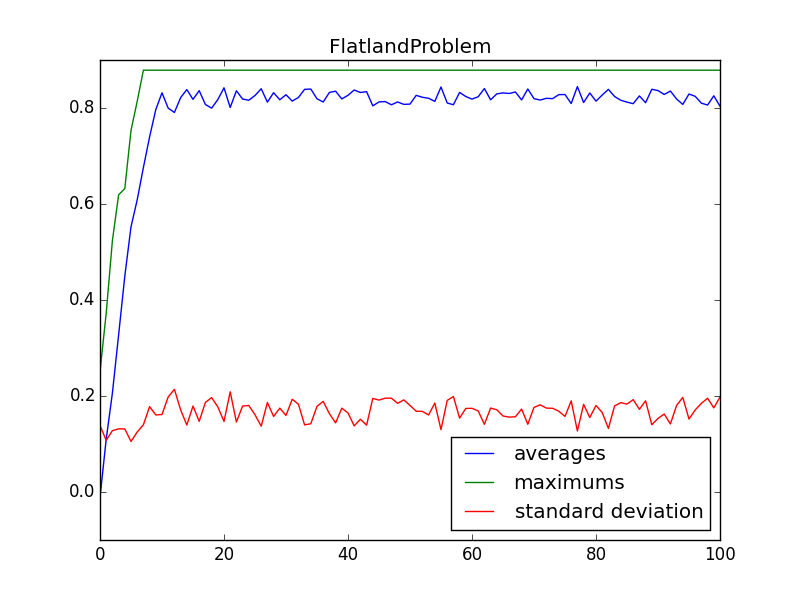
\includegraphics[width=\linewidth]{images/static_1.png}
    \caption{Fitness plot for static, single scenario run.} \label{fig:static-single}
  \end{figure}

  While no optimally performing agent was found,
  the best agent ate no poison and left only one piece of food in the static scenario.
  This resulted in a fitness value of \textasciitilde $0.89$.
  Testing that same agent on a freshly generated scenario yielded a fitness value of \textasciitilde $0.44$.
  Since we are ``training'' the network only on a single scenario,
  it is to be expected that it will not be a good general solution.
  This explains the drop in performance on the new scenario.
  
  \subsection{Static, five scenarios}

  \begin{figure}[H]
    \centering
    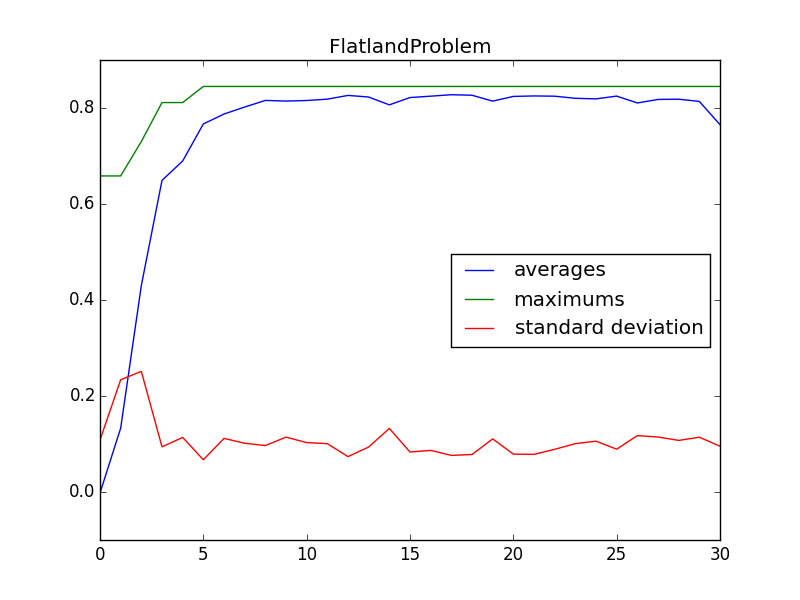
\includegraphics[width=\linewidth]{images/static_5.png}
    \caption{Fitness plot for static, five scenario per generation run.} \label{fig:static-single}
  \end{figure}

  Testing each generation on a static set of five scenarios does not yield a higher top fitness (\textasciitilde $0.85$).
  Applying the best individual on a new scenario resulted in a fitness of \textasciitilde $0.77$, which means this a slightly better strategy for breeding a general solution to the flatland-problem.
  Since the population is trained on the same set of scenarios each generation however,
  the generality of the resulting network depends on whether the five scenarios represent the breadth of the problem domain.
  If they are simillar then this training will not be much better than the single static scenario training.

  \subsection{Dynamic, single scenario}
  
  \begin{figure}[H]
    \centering
    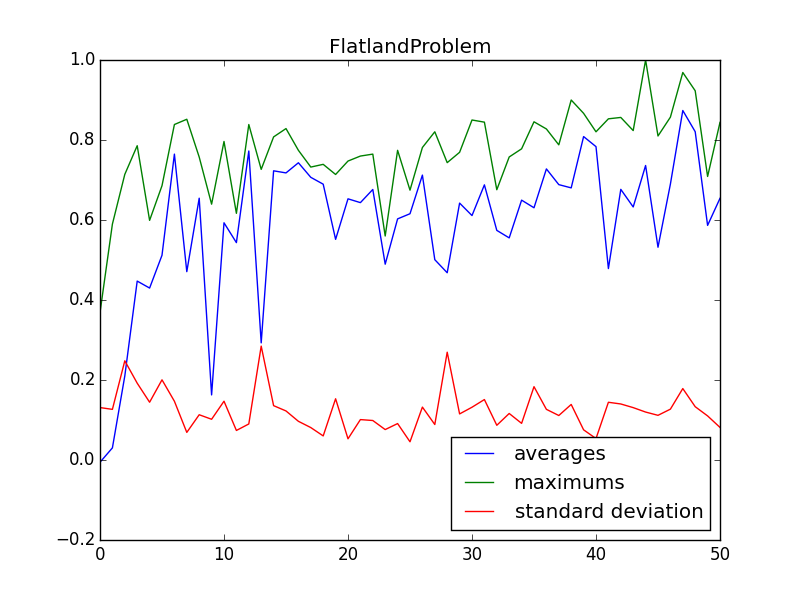
\includegraphics[width=\linewidth]{images/dynamic_1.png}
    \caption{Fitness plot for dynamic, single scenario run.} \label{fig:static-single}
  \end{figure}

  The dynamic, single scenario run has a very fluctuating finess plot.
  The ``environment'' changes too much for the selection pressure applied throughout the EA run have much value.

  The best performing individual scored a fitness value of \textasciitilde $0.98$ during the run, and \textasciitilde $0.57$ when retested on a new scenarios.

  \subsection{Dynamic, five scenarios}
  
  \begin{figure}[H]
    \centering
    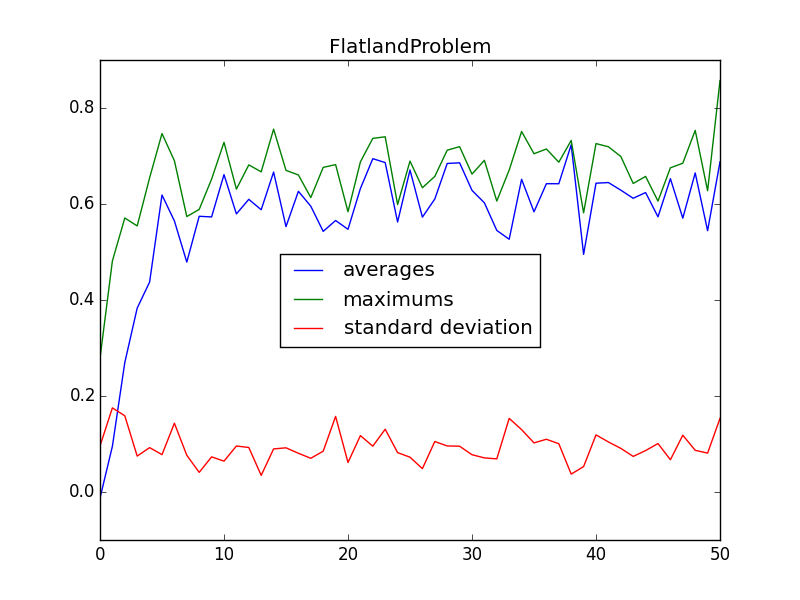
\includegraphics[width=\linewidth]{images/dynamic_5.png}
    \caption{Fitness plot for dynamic, five scenarios per generation.} \label{fig:static-single}
  \end{figure}

  As we can see from the figure, using a dynamic set of five scenarios yields a slightly less chaotic fitness plot.
  The best individual from this run scores a fitness value of \textasciitilde $0.86$.
  Retesting on a fresh board resulted in \textasciitilde $0.82$

  This is the best strategy for breeding agents that perform well in any instance of a flatland-problem.


\end{multicols}

%\bibliography{references}
%\bibliographystyle{plain}

\end{document}
